\section{Introduction}
\label{chapter:Introduction}

\textbf{Big Picture.}
The concept of object-oriented programming (OOP) is \textit{de facto standard} concept for developing large and complex 
applications because it provides inheritance for objects which are at first unrelated to each other; this in turn 
facilitates better code reuse, software maintenance and software design. There are many programing languages
which support OOP concepts, however the C++ programing language is the most used programming language for systems where 
runtime performance and reliability are key.

An important C++ OOP convention is the object calling convention when virtual functions are called.
Virtual functions are an important concept which facilitates late binding and allows the programmer to overwrite a
virtual function of the base-class with his own implementation. In fact, in order to implement virtual functions, 
the compiler needs to generate a table (\textit{i.e.,} virtual table meta-data structure) of all
virtual functions for each class containing them and provide to each instance of such a class (\textit{i.e.,} object) a pointer (\textit{i.e.,} virtual pointer)
to the aforementioned table. While this allows much more flexible code to be built---through late binding---it is simplistically implemented with no security
mechanisms at all.

\textbf{Problem.}
The performance benefit of late binding comes with high security implications. 
First, dangling object pointers lead to undefined behavior---as specified by the C++ language standard N4618~\cite{N4618}---which 
can be exploited to point into illegal (\textit{i.e.,} not previously intended) virtual tables.
Second, trough memory corruptions (\textit{e.g.,} buffer/integer overflows) the virtual pointer of an object making a 
call to a virtual function can be corrupted to point into:
\textit{1)} illegal virtual tables, 
\textit{2)} newly inserted virtual tables, or
\textit{3)} overwritten virtual table entries
such that advanced Code-Reuse Attacks (CRAs) as the recently published COOP~\cite{schuster:coop} 
and its extensions~\cite{crane:readactor++, crane:readactor++, subversive-c:lettner, ctf:coop, loop:oriented} 
become easily performable. This type of attack can bypass most of the to date CFI-based enforcement policies, since
\textit{1)} it does not exploit indirect backward edges (\textit{i.e.,} return edges) but rather
\textit{2)} it exploits the forward indirect control flow transfers imprecision which can not be upfront 
determined since alias analysis is undecidable~\cite{alias:undecidable}.

\textbf{Available Tools.}
To avoid object dispatch corruptions Control-Flow Integrity (CFI)~\cite{abadi:cfi2, abadi:cfi} can be successfully used.
CFI is one of the most used techniques for securing indirect control flow transfers inside programs
by usually adding runtime checks before each indirect call site.

Source code based tools usually insert runtime checks during the compilation of 
the program such as SafeDispatch~\cite{safedispatch:jang}, ShrinkWrap \cite{haller:shrinkwrap} and IFCC/VTV~\cite{vtv:tice}.
Other tools modify and reorder the contents of the virtual table layout such as VTI~\cite{bounov:interleaving} 
in order to derive efficient range checks on each object dispatch during runtime. Nevertheless, to the best of our knowledge 
due to runtime performance issues only IFCC/VTV~\cite{vtv:tice} is currently in production available.

Binary based tools typically enforce imprecise forward-edge CFI 
policies, often allowing control transfers from any valid call site 
to any valid referenced entry point \textit{e.g.,} binCFI~\cite{ccfir:zhang, zhang:usenix}. 
In the best case, existing policies only reduce the target set by
removing all entry points of other modules unless they were
explicitly exported or observed at runtime~\cite{payer:dimva}. 

TypeArmor~\cite{veen:typearmor} implements a fine grained forward edge CFI 
policy based on parameter count for binaries. It calculates invariants for call targets and indirect call sites based on
the number of parameters they use by leveraging static analysis of the binary, which then is
patched to enforce those invariants during runtime. 
The main shortcoming of TypeArmor is that it has low precision 
w.r.t. to the number of call targets allowed per call site 
(see \cref{{Too Permissive Parameter-Based Policies}} for more details).

VCI~\cite{vci:asiaccs} is a binary rewriting tool that can protect C++ binaries against 
vtable attacks. VCI strives to reconstruct several language semantics from the binary with limited success.
These will be later on used for a CFI policy based on resolving pairings of virtual table calls (vcall)
with precise sets of target classes. The policy is enforced similarly to TypeArmor by inserting the 
needed checks before each virtual call. VCI performs a restricted type of alias analysis during type propagation.
Also, it fails in some situations to identify the class types used by a vcall. Additionally, VCI can not deal with 
virtual-dispatch-like C calls and it fails to find any
constructor that defines the \textit{this} pointer. Overall, VCI tries to recuperate many high level 
semantics without focusing on one of them from the binary. As result the call target set per call site is too 
permissive.

\textbf{Tool Limitations.}
These source code tools offer a certain degree of protection when code is provided, however 
the above mentioned binary tools offer limited or no protection due to an imprecisely determined
call target set per call site.

\textbf{Our Idea.}
In this paper, we present \textsc{TypeShield}, a runtime illegitimate forward 
calls detection tool that is based on an improved forward-edge CFI policy compared to TypeArmor. 
\textsc{TypeShield} provides a more stricter set of allowed call targets per call site.
\textsc{TypeShield} is based on a use-def callees analysis to approximated the function prototypes, 
and liveness analysis at indirect callsites to approximate callsite signatures. This 
efficiently leads to a more precise CFG of the binary program in question, 
which can be used also by other systems in order to gain a more precise CFG on which to 
enforce other types of CFI related policies.
\textsc{TypeShield} incorporates an improved protection policy which is
based on the insight that if the binary adheres to the standard calling convention
for indirect calls, undefined arguments at the call site are not used by any callee by design. 
This further helps to reduce the possible target set of callees for each callsite.
\textsc{TypeShield} relies on a more precise than TypeArmor construction of both the callee parameter types and call site signatures.
\textsc{TypeShield} uses automatically inferred parameter types which are later used into the classification of matching call sites and call targets.
This helps to obtain more precise callee target sets for each caller as the TypeArmor.
\textsc{TypeShield} compared to TypeArmor uses different analysis strategies for basic block merging.
Furthermore, \textsc{TypeShield} disallows an indirect call transfer that prepares
fewer arguments than the target callee consumes and where the types of the 
arguments provided are not super types of the arguments expected at the target.
It then uses this information to enforce that each call site targets only a strict call target set.
\textsc{TypeShield} takes the binary of a program as input and it automatically instrument it in order
to detect illegitimate indirect calls at runtime. 
More precisely, \textsc{TypeShield} achieves three goals:
\begin{itemize}
 \item \textbf{Precision.} \textsc{TypeShield} employs a more precise analysis than TypeArmor in order to reduce the call target set for each 
               call site. Our evaluation shows that \textsc{TypeShield} incurs X\% precision w.r.t. TypeArmor on the same programs.
 \item \textbf{Performance.} \textsc{TypeShield} employs runtime policy optimization techniques to further reduce the runtime overheads
              Our evaluation shows that \textsc{TypeShield} imposes up to X\% and X\% overheads for performance-intensive benchmarks on the
              SPEC CPU2006 benchamrks and the webser applications, respectively. On
              the contrary, TypeArmor is X\% slower than \textsc{TypeShield}
              on the x Program.
 \item \textbf{Scope.} \textsc{TypeShield} can detect forbidden indirect calls and as such it can protect similarly as vTrust~\cite{zhang:vtrust} against
              virtual table injection, corruption and reuse attacks. As such \textsc{TypeShield} can serve as a platform for developing other types of defenses for different 
              types of attacks.
\end{itemize}

\textbf{Contributions.} 
In summary, we make the following contributions:
\label{Contribution}
\begin{itemize}
 \item \textbf{Security analysis of forward indirect calls.} 
 We analyzed the usage of illegitimate indirect forward calls in detail,
 thus providing security researchers and practitioners a better understanding of this emerging
 threat.

 \item \textbf{Illegitimate indirect calls detection tool.}
 We designed and implemented \textsc{TypeSchield}, a general, automated, and easy to deploy tool
 that can be applied to C/C++ binaries in order to detect and mitigate illegitimate forward indirect calls 
 during runtime. 
 
 \item \textbf{Experiments.} We demonstrate trough extensive experiments that our precise
 binary-level CFI strategy can mitigate advanced code reuse attacks in absence of C++ semantics.
 For example \textsc{TypeSchield} can protect against the COOP attack and its variations.
\end{itemize}

\newsavebox{\firstlisting}
\begin{lrbox}{\firstlisting}
\begin{minipage}[c]{\linewidth}
\begin{minted}[
% frame=lines,
framesep=2mm,
linenos,
frame=none,
firstnumber=1,
framesep = 1.0cm,
linenos,
numbersep=5pt,
%gobble=2,
%frame=lines,
framesep=2mm,
%fontsize=\tiny        
% baselinestretch=1.2,
% bgcolor=LightGray,
fontsize=\footnotesize,
]{C++}
class nsMultiplexInputStream final 
 :public nsIMultiplexInputStream //A0
 ,public nsISeekableStream //A1
 ,public nsIIPCSerializableInputStream //A2
 ,public nsICloneableInputStream{ //A3
nsTArray<nsCOMPtr<nsIInputStream>> mStreams;
NS_IMETHODIMP nsMultiplexInputStream::Close(){
  MutexAutoLock lock(mLock);
  mStatus = NS_BASE_STREAM_CLOSED;
  //set NS_OK flag
  nsresult rv = NS_OK;
  //get array length
  uint32_t len = mStreams.Length();
  //array-based main loop gadget
 for (uint32_t i = 0; i<len; ++i){
  //(1) hijacked indirect call
  nsresult rv2=mStreams[i]->Close();
  if (NS_FAILED(rv2)) {
      rv = rv2;
  }
 }
  return rv;
}
\end{minted}
\end{minipage}
\end{lrbox}

% \begin{figure}
%  \begin{minipage}[!t]{.40\linewidth}
%   \usebox{\firstlisting}
%  \end{minipage}%%
% \hfill
% \hspace{1.2cm}
% \begin{minipage}[!b]{.5\linewidth}
%    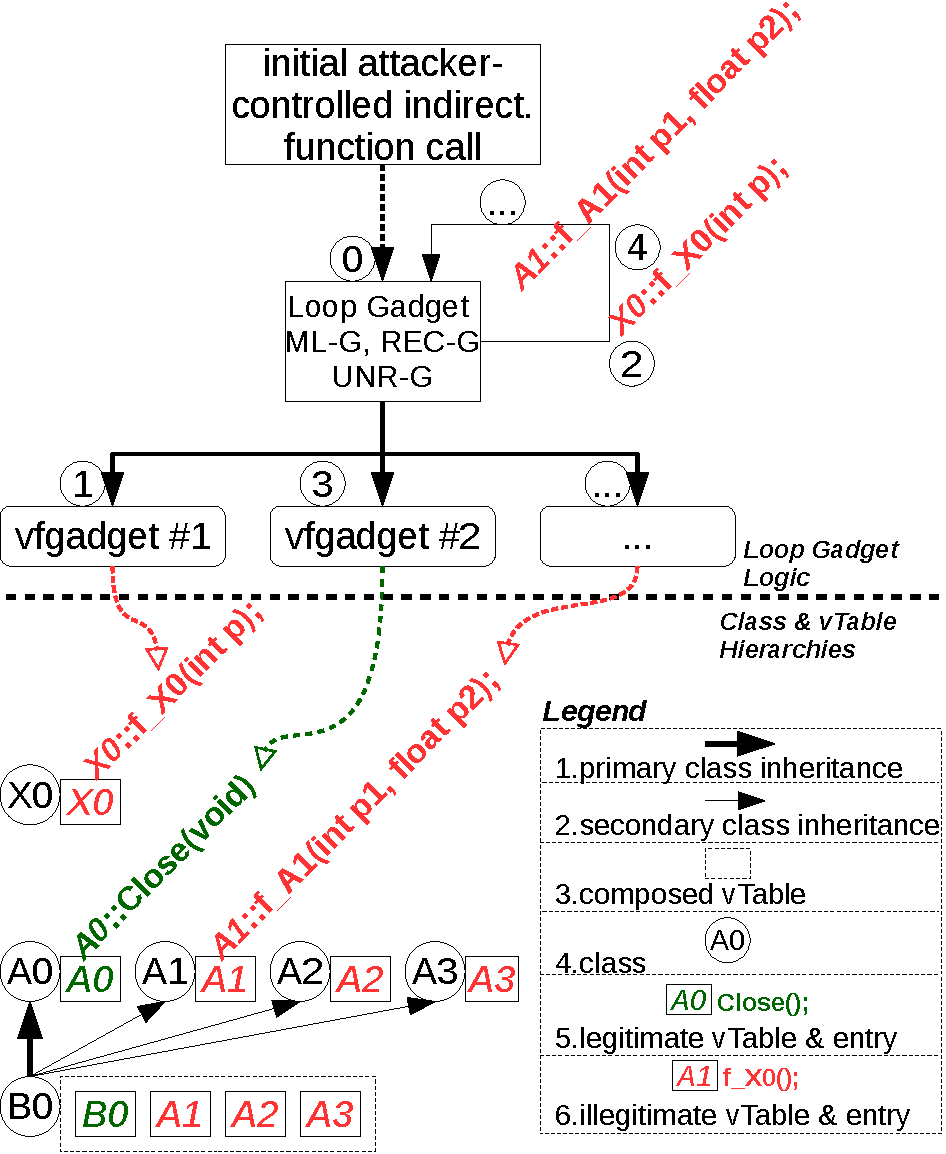
\includegraphics[width=1.3\textwidth]{figures/loop.pdf}
% \end{minipage}
% \caption{Code example used to illustrate how a COOP loop gadget works.}
% \label{Code example used to illustrate how a COOP loop gadget works}
% \end{figure}

%%%%%%%%%%%%%%%%%
 \begin{figure*}[!t]
   \setlength{\unitlength}{0.1\textwidth}
   \begin{picture}(10,4)
   \centering
     \put(4.51,0){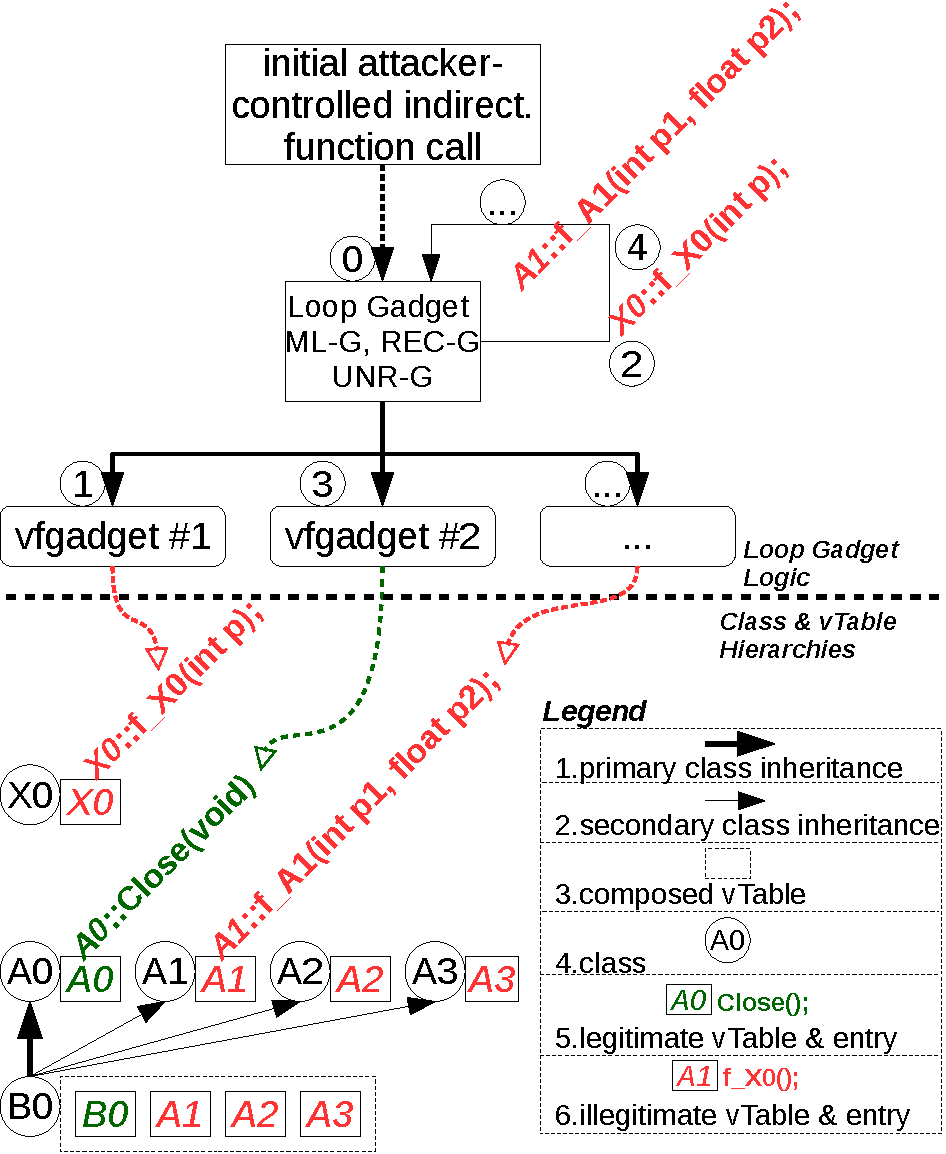
\includegraphics[width=.37\textwidth]{figures/loop.pdf}}
     \put(1.5,2){\usebox{\firstlisting}}
   \end{picture}
\caption{Graphic depicting how a COOP loop gadget works.}
\label{Code example used to illustrate how a COOP loop gadget works}
\end{figure*}

%most probably not needed at this time.
% \label{Outline}
% \textbf{Outline.} 
The remainder of this paper is organized as follows.
\cref{C++ Bad Forward Indirect Calls} explains forbidden forward indirect calls issues and their security implications.
\cref{chapter:TypeShild Overview} contains an overview of \textsc{TypeShield}.
\cref{chapter:Design} describes the theory used and decisions made during the design of \textsc{TypeShield}.
\cref{chapter:Implementation} briefly presents the implementation details of \textsc{TypeShield}.
\cref{chapter:Evaluation} evaluates several properties of \textsc{TypeShield} and
\cref{chapter:Related_Work} surveys related work, respectively.
\cref{chapter:Discussion} contains the discussion while 
\cref{chapter:Future_Work} highlights future research venues, respectively. 
Finally, \cref{chapter:Conclusion} concludes this paper.


